% multiple1902 <multiple1902@gmail.com>
% available on https://code.google.com/p/xjtu-cs-lect/
% licensed under cc by-sa 3.0
\setcounter{chapter}{-1}
\chapter{绪论}

\section{什么是组合数学}

    \textsf{组合数学}(combinatorial mathematics)是研究离散结构的存在, 计数, 分析和优化等问题的一门学科. 它

    \begin{itemize}
        \item (构造性)研究事物在给定模式下的配置(也称为方案),
        \item (存在性)研究这种配置(方案)是否存在
            \begin{itemize}
                \item 所有可能配置(方案)的数目和分类(计数),
                \item 配置(方案)的各种性质(优化).
            \end{itemize}
    \end{itemize}

\section{古代组合数学}

    组合数学源远流长, 但在远古时代这类问题往往联系着数的神秘主义出现. 

    \subsection{河图, 洛书}

        河图洛书, 来自上古时代有关数字排列之图案. 在宋朝之前, 洛书的记述只有文字, 一直到陈抟, 才提出了洛书的图案. 有人认为是重要的中国传统易理哲学部分, 后被广泛应用于风水、占卜等术数中. 
       
        \begin{figure}[!h]
            \centering
            \begin{minipage}[t]{.4\linewidth}
                \centering
                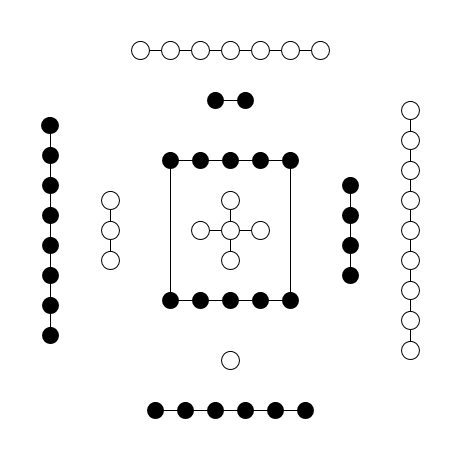
\includegraphics[width=.8\linewidth]{comb_notes/chap0_inc/河图.png}
                    % public domain
                \caption{河图}
                \label{fig:0:hetu}
            \end{minipage}
            \begin{minipage}[t]{.4\linewidth}
                \centering
                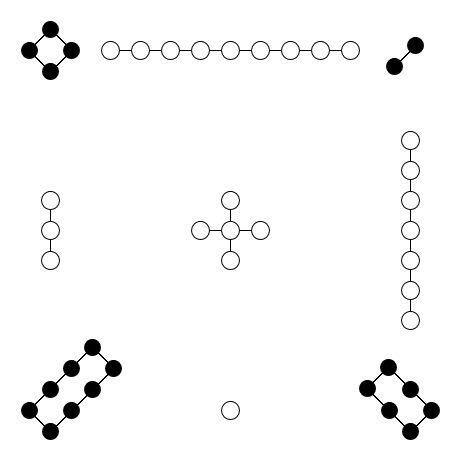
\includegraphics[width=.8\linewidth]{comb_notes/chap0_inc/洛书.png}
                    % public domain
                \caption{洛书}
                \label{fig:0:luoshu}
            \end{minipage}
        \end{figure}

        今人有人认为《河图》(图\ref{fig:0:hetu})是银河系双螺旋结构的数理模型.

        《洛书》实际上是一三阶幻方: \textsf{幻方}是每行、每列、主副对角线上数字之和全相等的方阵. $n$阶幻方的\textsf{幻和}$S_n=\frac{n(n^2+1)}{2}$.

        \subsubsection{奇数阶幻方的构造}

            \paragraph{劳伯尔算法}

                \begin{enumerate}
                    \item 在顶行(即第一行)中间写上数1,
                    \item 下一个数填写在前一个数的右上角位置上,
                    \item 当右上角不存在或已被填写时, 按下述规则修改之:
                        \begin{enumerate}
                            \item 当到达顶行时, 认为底行(即第$n$行)接在顶行之上;
                            \item 当到达最右列(即第$n$列)时, 认为最左列(即第一列)接在最右列之右;
                            \item 当欲填位置上已被填写, 或达到顶行最右列(即右上角)时, 下一个数填在前一个数的下边.
                        \end{enumerate}
                \end{enumerate}

            \paragraph{麦哲里克算法}

                \begin{enumerate}
                    \item 先在正中央方格的上方写上数1,
                    \setcounter{enumi}{2}
                    \item 
                        \begin{enumerate}
                            \setcounter{enumii}{2}
                            \item 当欲填位置上已被填写,或达到顶行最右列(即右上角)时,下一个数填在前一个数的上方两格处.
                        \end{enumerate}
                \end{enumerate}


